\documentclass[1p]{elsarticle_modified}
%\bibliographystyle{elsarticle-num}

%\usepackage[colorlinks]{hyperref}
%\usepackage{abbrmath_seonhwa} %\Abb, \Ascr, \Acal ,\Abf, \Afrak
\usepackage{amsfonts}
\usepackage{amssymb}
\usepackage{amsmath}
\usepackage{amsthm}
\usepackage{scalefnt}
\usepackage{amsbsy}
\usepackage{kotex}
\usepackage{caption}
\usepackage{subfig}
\usepackage{color}
\usepackage{graphicx}
\usepackage{xcolor} %% white, black, red, green, blue, cyan, magenta, yellow
\usepackage{float}
\usepackage{setspace}
\usepackage{hyperref}

\usepackage{tikz}
\usetikzlibrary{arrows}

\usepackage{multirow}
\usepackage{array} % fixed length table
\usepackage{hhline}

%%%%%%%%%%%%%%%%%%%%%
\makeatletter
\renewcommand*\env@matrix[1][\arraystretch]{%
	\edef\arraystretch{#1}%
	\hskip -\arraycolsep
	\let\@ifnextchar\new@ifnextchar
	\array{*\c@MaxMatrixCols c}}
\makeatother %https://tex.stackexchange.com/questions/14071/how-can-i-increase-the-line-spacing-in-a-matrix
%%%%%%%%%%%%%%%

\usepackage[normalem]{ulem}

\newcommand{\msout}[1]{\ifmmode\text{\sout{\ensuremath{#1}}}\else\sout{#1}\fi}
%SOURCE: \msout is \stkout macro in https://tex.stackexchange.com/questions/20609/strikeout-in-math-mode

\newcommand{\cancel}[1]{
	\ifmmode
	{\color{red}\msout{#1}}
	\else
	{\color{red}\sout{#1}}
	\fi
}

\newcommand{\add}[1]{
	{\color{blue}\uwave{#1}}
}

\newcommand{\replace}[2]{
	\ifmmode
	{\color{red}\msout{#1}}{\color{blue}\uwave{#2}}
	\else
	{\color{red}\sout{#1}}{\color{blue}\uwave{#2}}
	\fi
}

\newcommand{\Sol}{\mathcal{S}} %segment
\newcommand{\D}{D} %diagram
\newcommand{\A}{\mathcal{A}} %arc


%%%%%%%%%%%%%%%%%%%%%%%%%%%%%5 test

\def\sl{\operatorname{\textup{SL}}(2,\Cbb)}
\def\psl{\operatorname{\textup{PSL}}(2,\Cbb)}
\def\quan{\mkern 1mu \triangleright \mkern 1mu}

\theoremstyle{definition}
\newtheorem{thm}{Theorem}[section]
\newtheorem{prop}[thm]{Proposition}
\newtheorem{lem}[thm]{Lemma}
\newtheorem{ques}[thm]{Question}
\newtheorem{cor}[thm]{Corollary}
\newtheorem{defn}[thm]{Definition}
\newtheorem{exam}[thm]{Example}
\newtheorem{rmk}[thm]{Remark}
\newtheorem{alg}[thm]{Algorithm}

\newcommand{\I}{\sqrt{-1}}
\begin{document}

%\begin{frontmatter}
%
%\title{Boundary parabolic representations of knots up to 8 crossings}
%
%%% Group authors per affiliation:
%\author{Yunhi Cho} 
%\address{Department of Mathematics, University of Seoul, Seoul, Korea}
%\ead{yhcho@uos.ac.kr}
%
%
%\author{Seonhwa Kim} %\fnref{s_kim}}
%\address{Center for Geometry and Physics, Institute for Basic Science, Pohang, 37673, Korea}
%\ead{ryeona17@ibs.re.kr}
%
%\author{Hyuk Kim}
%\address{Department of Mathematical Sciences, Seoul National University, Seoul 08826, Korea}
%\ead{hyukkim@snu.ac.kr}
%
%\author{Seokbeom Yoon}
%\address{Department of Mathematical Sciences, Seoul National University, Seoul, 08826,  Korea}
%\ead{sbyoon15@snu.ac.kr}
%
%\begin{abstract}
%We find all boundary parabolic representation of knots up to 8 crossings.
%
%\end{abstract}
%\begin{keyword}
%    \MSC[2010] 57M25 
%\end{keyword}
%
%\end{frontmatter}

%\linenumbers
%\tableofcontents
%
\newcommand\colored[1]{\textcolor{white}{\rule[-0.35ex]{0.8em}{1.4ex}}\kern-0.8em\color{red} #1}%
%\newcommand\colored[1]{\textcolor{white}{ #1}\kern-2.17ex	\textcolor{white}{ #1}\kern-1.81ex	\textcolor{white}{ #1}\kern-2.15ex\color{red}#1	}

{\Large $\underline{12n_{0711}~(K12n_{0711})}$}

\setlength{\tabcolsep}{10pt}
\renewcommand{\arraystretch}{1.6}
\vspace{1cm}\begin{tabular}{m{100pt}>{\centering\arraybackslash}m{274pt}}
\multirow{5}{120pt}{
	\centering
	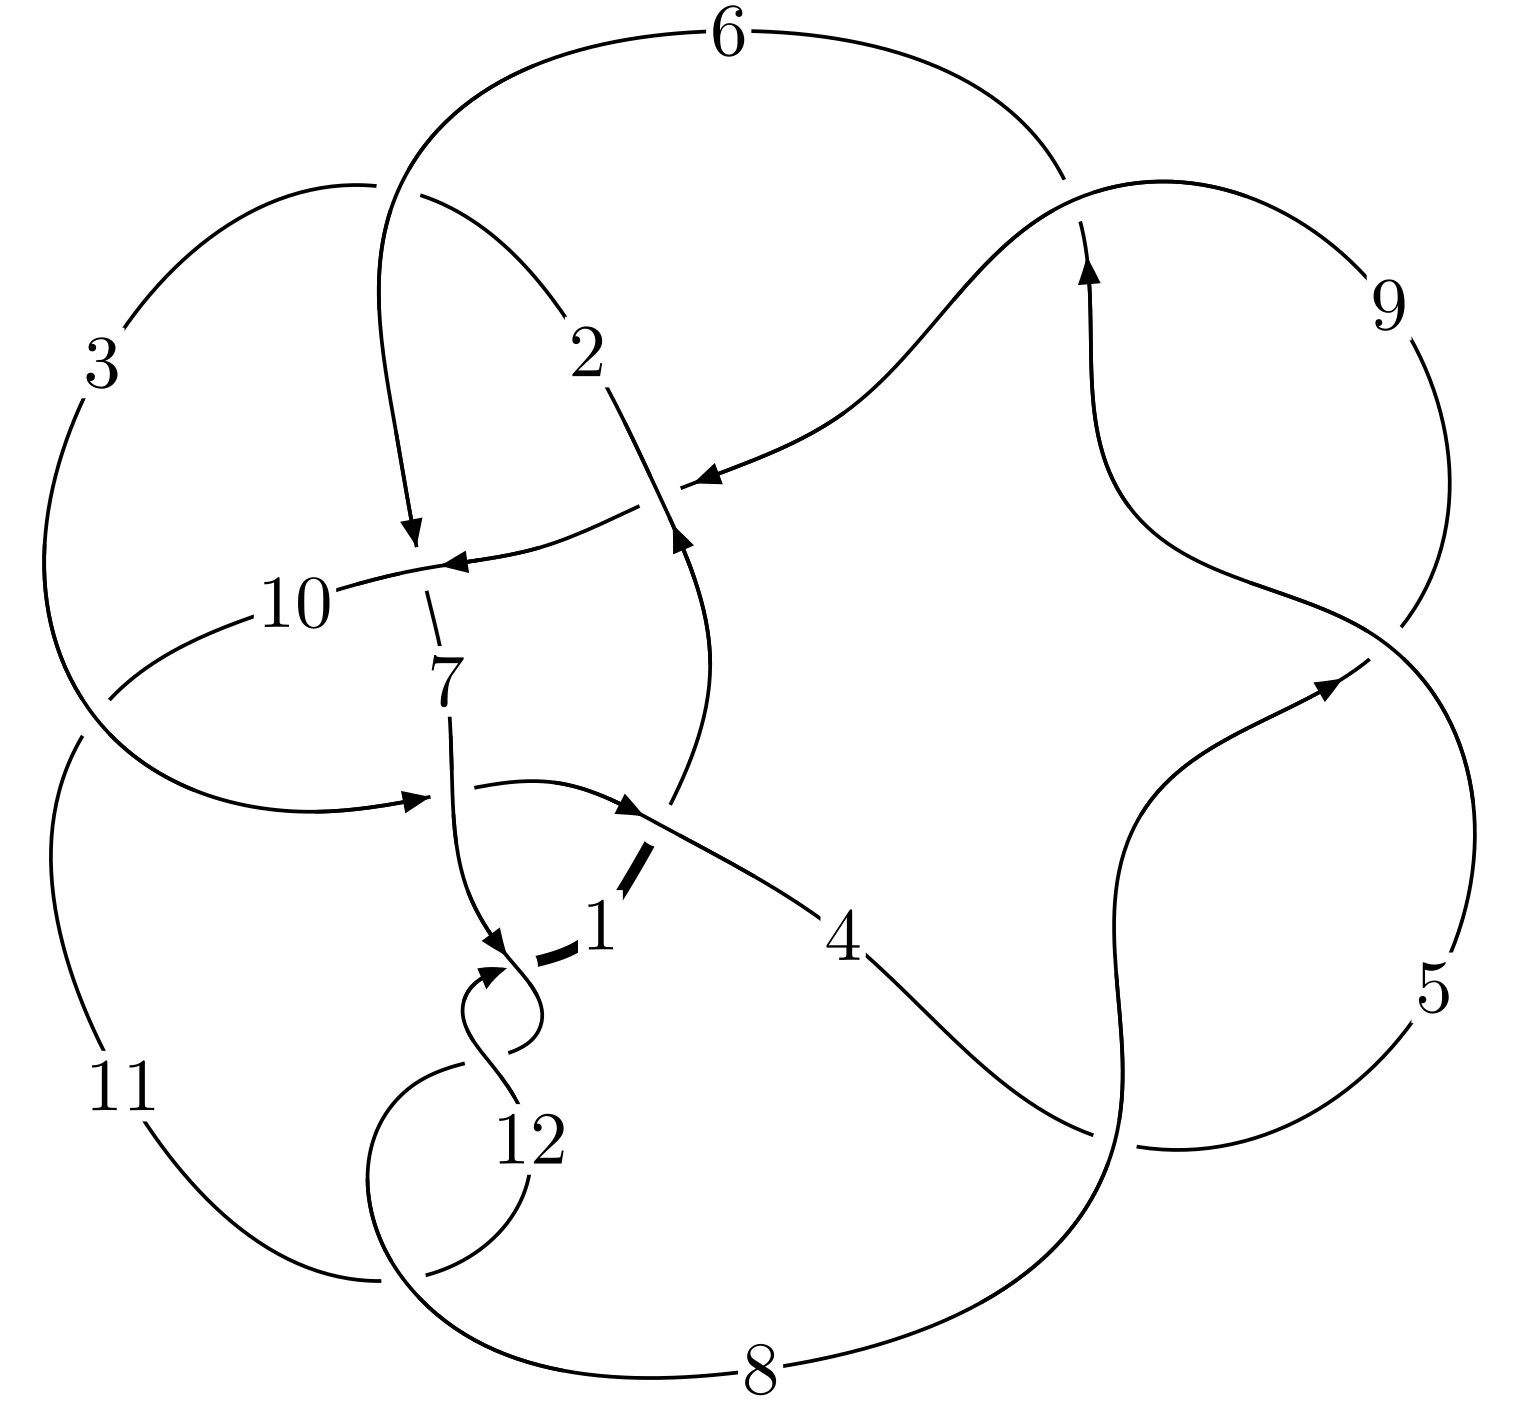
\includegraphics[width=112pt]{../../../GIT/diagram.site/Diagrams/png/2800_12n_0711.png}\\
\ \ \ A knot diagram\footnotemark}&
\allowdisplaybreaks
\textbf{Linearized knot diagam} \\
\cline{2-2}
 &
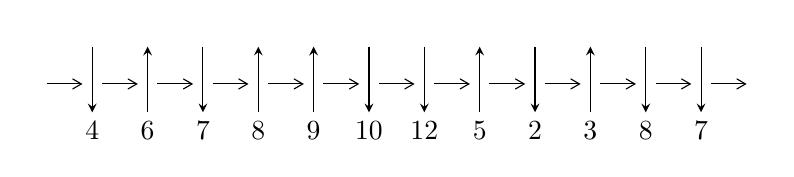
\begin{tikzpicture}[x=20pt, y=17pt]
	% nodes
	\node (C0) at (0, 0) {};
	\node (C1) at (1, 0) {};
	\node (C1U) at (1, +1) {};
	\node (C1D) at (1, -1) {4};

	\node (C2) at (2, 0) {};
	\node (C2U) at (2, +1) {};
	\node (C2D) at (2, -1) {6};

	\node (C3) at (3, 0) {};
	\node (C3U) at (3, +1) {};
	\node (C3D) at (3, -1) {7};

	\node (C4) at (4, 0) {};
	\node (C4U) at (4, +1) {};
	\node (C4D) at (4, -1) {8};

	\node (C5) at (5, 0) {};
	\node (C5U) at (5, +1) {};
	\node (C5D) at (5, -1) {9};

	\node (C6) at (6, 0) {};
	\node (C6U) at (6, +1) {};
	\node (C6D) at (6, -1) {10};

	\node (C7) at (7, 0) {};
	\node (C7U) at (7, +1) {};
	\node (C7D) at (7, -1) {12};

	\node (C8) at (8, 0) {};
	\node (C8U) at (8, +1) {};
	\node (C8D) at (8, -1) {5};

	\node (C9) at (9, 0) {};
	\node (C9U) at (9, +1) {};
	\node (C9D) at (9, -1) {2};

	\node (C10) at (10, 0) {};
	\node (C10U) at (10, +1) {};
	\node (C10D) at (10, -1) {3};

	\node (C11) at (11, 0) {};
	\node (C11U) at (11, +1) {};
	\node (C11D) at (11, -1) {8};

	\node (C12) at (12, 0) {};
	\node (C12U) at (12, +1) {};
	\node (C12D) at (12, -1) {7};
	\node (C13) at (13, 0) {};

	% arrows
	\draw[->,>={angle 60}]
	(C0) edge (C1) (C1) edge (C2) (C2) edge (C3) (C3) edge (C4) (C4) edge (C5) (C5) edge (C6) (C6) edge (C7) (C7) edge (C8) (C8) edge (C9) (C9) edge (C10) (C10) edge (C11) (C11) edge (C12) (C12) edge (C13) ;	\draw[->,>=stealth]
	(C1U) edge (C1D) (C2D) edge (C2U) (C3U) edge (C3D) (C4D) edge (C4U) (C5D) edge (C5U) (C6U) edge (C6D) (C7U) edge (C7D) (C8D) edge (C8U) (C9U) edge (C9D) (C10D) edge (C10U) (C11U) edge (C11D) (C12U) edge (C12D) ;
	\end{tikzpicture} \\
\hhline{~~} \\& 
\textbf{Solving Sequence} \\ \cline{2-2} 
 &
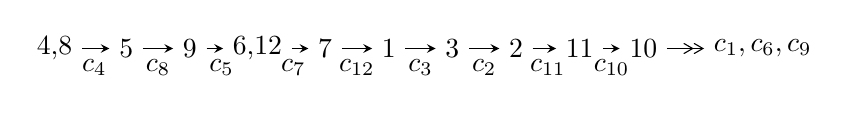
\begin{tikzpicture}[x=23pt, y=7pt]
	% node
	\node (A0) at (-1/8, 0) {4,8};
	\node (A1) at (1, 0) {5};
	\node (A2) at (2, 0) {9};
	\node (A3) at (49/16, 0) {6,12};
	\node (A4) at (33/8, 0) {7};
	\node (A5) at (41/8, 0) {1};
	\node (A6) at (49/8, 0) {3};
	\node (A7) at (57/8, 0) {2};
	\node (A8) at (65/8, 0) {11};
	\node (A9) at (73/8, 0) {10};
	\node (C1) at (1/2, -1) {$c_{4}$};
	\node (C2) at (3/2, -1) {$c_{8}$};
	\node (C3) at (5/2, -1) {$c_{5}$};
	\node (C4) at (29/8, -1) {$c_{7}$};
	\node (C5) at (37/8, -1) {$c_{12}$};
	\node (C6) at (45/8, -1) {$c_{3}$};
	\node (C7) at (53/8, -1) {$c_{2}$};
	\node (C8) at (61/8, -1) {$c_{11}$};
	\node (C9) at (69/8, -1) {$c_{10}$};
	\node (A10) at (11, 0) {$c_{1},c_{6},c_{9}$};

	% edge
	\draw[->,>=stealth]	
	(A0) edge (A1) (A1) edge (A2) (A2) edge (A3) (A3) edge (A4) (A4) edge (A5) (A5) edge (A6) (A6) edge (A7) (A7) edge (A8) (A8) edge (A9) ;
	\draw[->>,>={angle 60}]	
	(A9) edge (A10);
\end{tikzpicture} \\ 

\end{tabular} \\

\footnotetext{
The image of knot diagram is generated by the software ``\textbf{Draw programme}" developed by Andrew Bartholomew(\url{http://www.layer8.co.uk/maths/draw/index.htm\#Running-draw}), where we modified some parts for our purpose(\url{https://github.com/CATsTAILs/LinksPainter}).
}\phantom \\ \newline 
\centering \textbf{Ideals for irreducible components\footnotemark of $X_{\text{par}}$} 
 
\begin{align*}
I^u_{1}&=\langle 
-1.02480\times10^{144} u^{75}+2.72391\times10^{145} u^{74}+\cdots+1.00707\times10^{147} b-2.72299\times10^{147},\\
\phantom{I^u_{1}}&\phantom{= \langle  }-1.35943\times10^{147} u^{75}-2.53685\times10^{147} u^{74}+\cdots+2.71908\times10^{148} a+9.43984\times10^{148},\\
\phantom{I^u_{1}}&\phantom{= \langle  }u^{76}+2 u^{75}+\cdots+32 u+27\rangle \\
I^u_{2}&=\langle 
28 u^{19}+35 u^{18}+\cdots+67 b+22,\;15 u^{19}+2 u^{18}+\cdots+67 a-194,\;u^{20}+u^{19}+\cdots+4 u^2+1\rangle \\
\\
\end{align*}
\raggedright * 2 irreducible components of $\dim_{\mathbb{C}}=0$, with total 96 representations.\\
\footnotetext{All coefficients of polynomials are rational numbers. But the coefficients are sometimes approximated in decimal forms when there is not enough margin.}
\newpage
\renewcommand{\arraystretch}{1}
\centering \section*{I. $I^u_{1}= \langle -1.02\times10^{144} u^{75}+2.72\times10^{145} u^{74}+\cdots+1.01\times10^{147} b-2.72\times10^{147},\;-1.36\times10^{147} u^{75}-2.54\times10^{147} u^{74}+\cdots+2.72\times10^{148} a+9.44\times10^{148},\;u^{76}+2 u^{75}+\cdots+32 u+27 \rangle$}
\flushleft \textbf{(i) Arc colorings}\\
\begin{tabular}{m{7pt} m{180pt} m{7pt} m{180pt} }
\flushright $a_{4}=$&$\begin{pmatrix}1\\0\end{pmatrix}$ \\
\flushright $a_{8}=$&$\begin{pmatrix}0\\u\end{pmatrix}$ \\
\flushright $a_{5}=$&$\begin{pmatrix}1\\- u^2\end{pmatrix}$ \\
\flushright $a_{9}=$&$\begin{pmatrix}u\\- u^3+u\end{pmatrix}$ \\
\flushright $a_{6}=$&$\begin{pmatrix}- u^2+1\\u^4-2 u^2\end{pmatrix}$ \\
\flushright $a_{12}=$&$\begin{pmatrix}0.0499959 u^{75}+0.0932981 u^{74}+\cdots+14.5526 u-3.47170\\0.00101760 u^{75}-0.0270480 u^{74}+\cdots+9.57085 u+2.70389\end{pmatrix}$ \\
\flushright $a_{7}=$&$\begin{pmatrix}-0.0527844 u^{75}+0.0417033 u^{74}+\cdots+27.5284 u+7.01584\\-0.0139024 u^{75}-0.0236058 u^{74}+\cdots-5.70988 u+2.14183\end{pmatrix}$ \\
\flushright $a_{1}=$&$\begin{pmatrix}-0.157862 u^{75}-0.367093 u^{74}+\cdots-8.05823 u+2.08138\\-0.0836878 u^{75}-0.135451 u^{74}+\cdots+2.18214 u+0.663016\end{pmatrix}$ \\
\flushright $a_{3}=$&$\begin{pmatrix}-0.0612921 u^{75}-0.196218 u^{74}+\cdots-0.851626 u+2.23369\\-0.0359843 u^{75}-0.0719567 u^{74}+\cdots+3.76665 u+1.20983\end{pmatrix}$ \\
\flushright $a_{2}=$&$\begin{pmatrix}-0.0741741 u^{75}-0.231641 u^{74}+\cdots-10.2404 u+1.41836\\-0.0836878 u^{75}-0.135451 u^{74}+\cdots+2.18214 u+0.663016\end{pmatrix}$ \\
\flushright $a_{11}=$&$\begin{pmatrix}0.0499959 u^{75}+0.0932981 u^{74}+\cdots+14.5526 u-3.47170\\0.0136984 u^{75}+0.00972375 u^{74}+\cdots+10.7065 u+2.52316\end{pmatrix}$ \\
\flushright $a_{10}=$&$\begin{pmatrix}0.0242324 u^{75}+0.132596 u^{74}+\cdots+2.52604 u-10.7945\\0.110043 u^{75}+0.116092 u^{74}+\cdots-5.22698 u-0.286295\end{pmatrix}$\\&\end{tabular}
\flushleft \textbf{(ii) Obstruction class $= -1$}\\~\\
\flushleft \textbf{(iii) Cusp Shapes $= 0.351617 u^{75}+0.565791 u^{74}+\cdots+64.9845 u+17.3733$}\\~\\
\newpage\renewcommand{\arraystretch}{1}
\flushleft \textbf{(iv) u-Polynomials at the component}\newline \\
\begin{tabular}{m{50pt}|m{274pt}}
Crossings & \hspace{64pt}u-Polynomials at each crossing \\
\hline $$\begin{aligned}c_{1}\end{aligned}$$&$\begin{aligned}
&u^{76}+5 u^{75}+\cdots-9804 u+1444
\end{aligned}$\\
\hline $$\begin{aligned}c_{2}\end{aligned}$$&$\begin{aligned}
&u^{76}-5 u^{75}+\cdots-124 u-23
\end{aligned}$\\
\hline $$\begin{aligned}c_{3}\end{aligned}$$&$\begin{aligned}
&u^{76}-2 u^{75}+\cdots+76 u+2633
\end{aligned}$\\
\hline $$\begin{aligned}c_{4},c_{5},c_{8}\end{aligned}$$&$\begin{aligned}
&u^{76}-2 u^{75}+\cdots-32 u+27
\end{aligned}$\\
\hline $$\begin{aligned}c_{6}\end{aligned}$$&$\begin{aligned}
&u^{76}-9 u^{74}+\cdots-22 u+19
\end{aligned}$\\
\hline $$\begin{aligned}c_{7},c_{11},c_{12}\end{aligned}$$&$\begin{aligned}
&u^{76}+13 u^{74}+\cdots-82 u+43
\end{aligned}$\\
\hline $$\begin{aligned}c_{9}\end{aligned}$$&$\begin{aligned}
&u^{76}-3 u^{75}+\cdots-397 u+71
\end{aligned}$\\
\hline $$\begin{aligned}c_{10}\end{aligned}$$&$\begin{aligned}
&u^{76}-3 u^{75}+\cdots+1147 u+447
\end{aligned}$\\
\hline
\end{tabular}\\~\\
\newpage\renewcommand{\arraystretch}{1}
\flushleft \textbf{(v) Riley Polynomials at the component}\newline \\
\begin{tabular}{m{50pt}|m{274pt}}
Crossings & \hspace{64pt}Riley Polynomials at each crossing \\
\hline $$\begin{aligned}c_{1}\end{aligned}$$&$\begin{aligned}
&y^{76}-67 y^{75}+\cdots+4349328 y+2085136
\end{aligned}$\\
\hline $$\begin{aligned}c_{2}\end{aligned}$$&$\begin{aligned}
&y^{76}-19 y^{75}+\cdots-82030 y+529
\end{aligned}$\\
\hline $$\begin{aligned}c_{3}\end{aligned}$$&$\begin{aligned}
&y^{76}-62 y^{75}+\cdots-205858982 y+6932689
\end{aligned}$\\
\hline $$\begin{aligned}c_{4},c_{5},c_{8}\end{aligned}$$&$\begin{aligned}
&y^{76}-76 y^{75}+\cdots+52976 y+729
\end{aligned}$\\
\hline $$\begin{aligned}c_{6}\end{aligned}$$&$\begin{aligned}
&y^{76}-18 y^{75}+\cdots-15152 y+361
\end{aligned}$\\
\hline $$\begin{aligned}c_{7},c_{11},c_{12}\end{aligned}$$&$\begin{aligned}
&y^{76}+26 y^{75}+\cdots+34556 y+1849
\end{aligned}$\\
\hline $$\begin{aligned}c_{9}\end{aligned}$$&$\begin{aligned}
&y^{76}+15 y^{75}+\cdots+88335 y+5041
\end{aligned}$\\
\hline $$\begin{aligned}c_{10}\end{aligned}$$&$\begin{aligned}
&y^{76}+13 y^{75}+\cdots+10810607 y+199809
\end{aligned}$\\
\hline
\end{tabular}\\~\\
\newpage\flushleft \textbf{(vi) Complex Volumes and Cusp Shapes}
$$\begin{array}{c|c|c}  
\text{Solutions to }I^u_{1}& \I (\text{vol} + \sqrt{-1}CS) & \text{Cusp shape}\\
 \hline 
\begin{aligned}
u &= -0.335219 + 0.952463 I \\
a &= \phantom{-}1.062340 + 0.659919 I \\
b &= \phantom{-}0.150378 + 1.163430 I\end{aligned}
 & -5.21982 - 4.95583 I & \phantom{-0.000000 } 0 \\ \hline\begin{aligned}
u &= -0.335219 - 0.952463 I \\
a &= \phantom{-}1.062340 - 0.659919 I \\
b &= \phantom{-}0.150378 - 1.163430 I\end{aligned}
 & -5.21982 + 4.95583 I & \phantom{-0.000000 } 0 \\ \hline\begin{aligned}
u &= -0.178055 + 0.889122 I \\
a &= -0.666647 + 0.389184 I \\
b &= -1.159090 + 0.249170 I\end{aligned}
 & \phantom{-}1.66667 - 4.02641 I & \phantom{-0.000000 -}0. + 11.13609 I \\ \hline\begin{aligned}
u &= -0.178055 - 0.889122 I \\
a &= -0.666647 - 0.389184 I \\
b &= -1.159090 - 0.249170 I\end{aligned}
 & \phantom{-}1.66667 + 4.02641 I & \phantom{-0.000000 } 0. - 11.13609 I \\ \hline\begin{aligned}
u &= \phantom{-}0.525368 + 0.975309 I \\
a &= \phantom{-}0.462645 + 1.130730 I \\
b &= \phantom{-}0.78335 + 1.42794 I\end{aligned}
 & -4.41523 + 11.68720 I & \phantom{-0.000000 } 0 \\ \hline\begin{aligned}
u &= \phantom{-}0.525368 - 0.975309 I \\
a &= \phantom{-}0.462645 - 1.130730 I \\
b &= \phantom{-}0.78335 - 1.42794 I\end{aligned}
 & -4.41523 - 11.68720 I & \phantom{-0.000000 } 0 \\ \hline\begin{aligned}
u &= -0.711614 + 0.490004 I \\
a &= \phantom{-}0.611255 - 0.464779 I \\
b &= \phantom{-}0.181183 - 0.021532 I\end{aligned}
 & \phantom{-}1.27366 - 1.54173 I & \phantom{-}3.50559 + 0. I\phantom{ +0.000000I} \\ \hline\begin{aligned}
u &= -0.711614 - 0.490004 I \\
a &= \phantom{-}0.611255 + 0.464779 I \\
b &= \phantom{-}0.181183 + 0.021532 I\end{aligned}
 & \phantom{-}1.27366 + 1.54173 I & \phantom{-}3.50559 + 0. I\phantom{ +0.000000I} \\ \hline\begin{aligned}
u &= \phantom{-}1.14400\phantom{ +0.000000I} \\
a &= -0.948499\phantom{ +0.000000I} \\
b &= -0.215745\phantom{ +0.000000I}\end{aligned}
 & -2.20411\phantom{ +0.000000I} & \phantom{-0.000000 } 0 \\ \hline\begin{aligned}
u &= -0.202334 + 1.146190 I \\
a &= \phantom{-}0.647997 - 0.848827 I \\
b &= \phantom{-}0.430923 - 1.278420 I\end{aligned}
 & -1.76191 - 3.13440 I & \phantom{-0.000000 } 0\\
 \hline 
 \end{array}$$\newpage$$\begin{array}{c|c|c}  
\text{Solutions to }I^u_{1}& \I (\text{vol} + \sqrt{-1}CS) & \text{Cusp shape}\\
 \hline 
\begin{aligned}
u &= -0.202334 - 1.146190 I \\
a &= \phantom{-}0.647997 + 0.848827 I \\
b &= \phantom{-}0.430923 + 1.278420 I\end{aligned}
 & -1.76191 + 3.13440 I & \phantom{-0.000000 } 0 \\ \hline\begin{aligned}
u &= -1.174240 + 0.252442 I \\
a &= -0.611112 + 0.449227 I \\
b &= -0.396824 - 0.716749 I\end{aligned}
 & -1.05451 + 1.17178 I & \phantom{-0.000000 } 0 \\ \hline\begin{aligned}
u &= -1.174240 - 0.252442 I \\
a &= -0.611112 - 0.449227 I \\
b &= -0.396824 + 0.716749 I\end{aligned}
 & -1.05451 - 1.17178 I & \phantom{-0.000000 } 0 \\ \hline\begin{aligned}
u &= \phantom{-}1.238270 + 0.109890 I \\
a &= -0.926139 - 0.563020 I \\
b &= \phantom{-}0.184791 + 0.103677 I\end{aligned}
 & -0.15602 - 2.47239 I & \phantom{-0.000000 } 0 \\ \hline\begin{aligned}
u &= \phantom{-}1.238270 - 0.109890 I \\
a &= -0.926139 + 0.563020 I \\
b &= \phantom{-}0.184791 - 0.103677 I\end{aligned}
 & -0.15602 + 2.47239 I & \phantom{-0.000000 } 0 \\ \hline\begin{aligned}
u &= \phantom{-}0.747450\phantom{ +0.000000I} \\
a &= -0.637437\phantom{ +0.000000I} \\
b &= -0.905014\phantom{ +0.000000I}\end{aligned}
 & -2.42462\phantom{ +0.000000I} & -4.01110\phantom{ +0.000000I} \\ \hline\begin{aligned}
u &= \phantom{-}0.634961 + 0.372638 I \\
a &= -0.314128 + 0.853405 I \\
b &= -0.091984 + 1.090970 I\end{aligned}
 & \phantom{-}0.16002 + 4.03023 I & -2.04460 - 10.11479 I \\ \hline\begin{aligned}
u &= \phantom{-}0.634961 - 0.372638 I \\
a &= -0.314128 - 0.853405 I \\
b &= -0.091984 - 1.090970 I\end{aligned}
 & \phantom{-}0.16002 - 4.03023 I & -2.04460 + 10.11479 I \\ \hline\begin{aligned}
u &= -1.257720 + 0.166055 I \\
a &= -0.746919 + 0.518415 I \\
b &= \phantom{-}0.399959 - 0.632265 I\end{aligned}
 & -0.450371 - 1.016900 I & \phantom{-0.000000 } 0 \\ \hline\begin{aligned}
u &= -1.257720 - 0.166055 I \\
a &= -0.746919 - 0.518415 I \\
b &= \phantom{-}0.399959 + 0.632265 I\end{aligned}
 & -0.450371 + 1.016900 I & \phantom{-0.000000 } 0\\
 \hline 
 \end{array}$$\newpage$$\begin{array}{c|c|c}  
\text{Solutions to }I^u_{1}& \I (\text{vol} + \sqrt{-1}CS) & \text{Cusp shape}\\
 \hline 
\begin{aligned}
u &= \phantom{-}0.789767 + 1.016560 I \\
a &= \phantom{-}0.923614 - 0.121588 I \\
b &= \phantom{-}0.088501 - 0.909369 I\end{aligned}
 & -3.79850 - 5.20157 I & \phantom{-0.000000 } 0 \\ \hline\begin{aligned}
u &= \phantom{-}0.789767 - 1.016560 I \\
a &= \phantom{-}0.923614 + 0.121588 I \\
b &= \phantom{-}0.088501 + 0.909369 I\end{aligned}
 & -3.79850 + 5.20157 I & \phantom{-0.000000 } 0 \\ \hline\begin{aligned}
u &= -1.014430 + 0.821372 I \\
a &= -0.011572 - 0.978844 I \\
b &= \phantom{-}0.77138 - 1.60224 I\end{aligned}
 & -3.37044 - 1.02943 I & \phantom{-0.000000 } 0 \\ \hline\begin{aligned}
u &= -1.014430 - 0.821372 I \\
a &= -0.011572 + 0.978844 I \\
b &= \phantom{-}0.77138 + 1.60224 I\end{aligned}
 & -3.37044 + 1.02943 I & \phantom{-0.000000 } 0 \\ \hline\begin{aligned}
u &= \phantom{-}1.354330 + 0.034566 I \\
a &= -0.355159 - 0.633725 I \\
b &= \phantom{-}1.72523 - 0.83396 I\end{aligned}
 & \phantom{-}6.59906 - 2.06008 I & \phantom{-0.000000 } 0 \\ \hline\begin{aligned}
u &= \phantom{-}1.354330 - 0.034566 I \\
a &= -0.355159 + 0.633725 I \\
b &= \phantom{-}1.72523 + 0.83396 I\end{aligned}
 & \phantom{-}6.59906 + 2.06008 I & \phantom{-0.000000 } 0 \\ \hline\begin{aligned}
u &= -1.352470 + 0.091220 I \\
a &= -0.452501 + 0.509412 I \\
b &= \phantom{-}2.09424 + 0.03971 I\end{aligned}
 & \phantom{-}6.22160 - 3.70134 I & \phantom{-0.000000 } 0 \\ \hline\begin{aligned}
u &= -1.352470 - 0.091220 I \\
a &= -0.452501 - 0.509412 I \\
b &= \phantom{-}2.09424 - 0.03971 I\end{aligned}
 & \phantom{-}6.22160 + 3.70134 I & \phantom{-0.000000 } 0 \\ \hline\begin{aligned}
u &= \phantom{-}1.354550 + 0.202068 I \\
a &= \phantom{-}0.461925 - 0.797105 I \\
b &= -1.87703 - 1.23809 I\end{aligned}
 & \phantom{-}0.19010 + 7.12458 I & \phantom{-0.000000 } 0 \\ \hline\begin{aligned}
u &= \phantom{-}1.354550 - 0.202068 I \\
a &= \phantom{-}0.461925 + 0.797105 I \\
b &= -1.87703 + 1.23809 I\end{aligned}
 & \phantom{-}0.19010 - 7.12458 I & \phantom{-0.000000 } 0\\
 \hline 
 \end{array}$$\newpage$$\begin{array}{c|c|c}  
\text{Solutions to }I^u_{1}& \I (\text{vol} + \sqrt{-1}CS) & \text{Cusp shape}\\
 \hline 
\begin{aligned}
u &= \phantom{-}1.364060 + 0.156000 I \\
a &= \phantom{-}0.327441 - 0.829687 I \\
b &= -1.29343 - 2.14767 I\end{aligned}
 & \phantom{-}0.29364 + 3.54039 I & \phantom{-0.000000 } 0 \\ \hline\begin{aligned}
u &= \phantom{-}1.364060 - 0.156000 I \\
a &= \phantom{-}0.327441 + 0.829687 I \\
b &= -1.29343 + 2.14767 I\end{aligned}
 & \phantom{-}0.29364 - 3.54039 I & \phantom{-0.000000 } 0 \\ \hline\begin{aligned}
u &= \phantom{-}1.356250 + 0.217693 I \\
a &= -0.339965 - 0.976740 I \\
b &= \phantom{-}0.439699 - 1.333720 I\end{aligned}
 & \phantom{-}8.27803 - 1.11792 I & \phantom{-0.000000 } 0 \\ \hline\begin{aligned}
u &= \phantom{-}1.356250 - 0.217693 I \\
a &= -0.339965 + 0.976740 I \\
b &= \phantom{-}0.439699 + 1.333720 I\end{aligned}
 & \phantom{-}8.27803 + 1.11792 I & \phantom{-0.000000 } 0 \\ \hline\begin{aligned}
u &= -1.371200 + 0.168132 I \\
a &= -0.130034 + 1.111990 I \\
b &= -0.01517 + 1.48792 I\end{aligned}
 & \phantom{-}8.82106 - 5.99255 I & \phantom{-0.000000 } 0 \\ \hline\begin{aligned}
u &= -1.371200 - 0.168132 I \\
a &= -0.130034 - 1.111990 I \\
b &= -0.01517 - 1.48792 I\end{aligned}
 & \phantom{-}8.82106 + 5.99255 I & \phantom{-0.000000 } 0 \\ \hline\begin{aligned}
u &= -1.382190 + 0.164386 I \\
a &= \phantom{-}0.440963 + 1.011550 I \\
b &= -1.01477 + 1.50773 I\end{aligned}
 & \phantom{-}1.31274 - 6.74682 I & \phantom{-0.000000 } 0 \\ \hline\begin{aligned}
u &= -1.382190 - 0.164386 I \\
a &= \phantom{-}0.440963 - 1.011550 I \\
b &= -1.01477 - 1.50773 I\end{aligned}
 & \phantom{-}1.31274 + 6.74682 I & \phantom{-0.000000 } 0 \\ \hline\begin{aligned}
u &= -0.450364 + 0.405755 I \\
a &= \phantom{-}0.601796 - 1.157140 I \\
b &= \phantom{-}0.496255 - 0.470062 I\end{aligned}
 & \phantom{-}0.64900 - 1.50177 I & \phantom{-}0.08009 + 5.08857 I \\ \hline\begin{aligned}
u &= -0.450364 - 0.405755 I \\
a &= \phantom{-}0.601796 + 1.157140 I \\
b &= \phantom{-}0.496255 + 0.470062 I\end{aligned}
 & \phantom{-}0.64900 + 1.50177 I & \phantom{-}0.08009 - 5.08857 I\\
 \hline 
 \end{array}$$\newpage$$\begin{array}{c|c|c}  
\text{Solutions to }I^u_{1}& \I (\text{vol} + \sqrt{-1}CS) & \text{Cusp shape}\\
 \hline 
\begin{aligned}
u &= -0.085145 + 0.597383 I \\
a &= -1.24522 + 1.45142 I \\
b &= -0.99539 + 1.09484 I\end{aligned}
 & -4.39381 - 4.30048 I & -8.88569 + 7.94405 I \\ \hline\begin{aligned}
u &= -0.085145 - 0.597383 I \\
a &= -1.24522 - 1.45142 I \\
b &= -0.99539 - 1.09484 I\end{aligned}
 & -4.39381 + 4.30048 I & -8.88569 - 7.94405 I \\ \hline\begin{aligned}
u &= -1.394540 + 0.190085 I \\
a &= \phantom{-}0.600186 + 0.805977 I \\
b &= -1.27776 + 1.08700 I\end{aligned}
 & \phantom{-}0.45871 - 4.89022 I & \phantom{-0.000000 } 0 \\ \hline\begin{aligned}
u &= -1.394540 - 0.190085 I \\
a &= \phantom{-}0.600186 - 0.805977 I \\
b &= -1.27776 - 1.08700 I\end{aligned}
 & \phantom{-}0.45871 + 4.89022 I & \phantom{-0.000000 } 0 \\ \hline\begin{aligned}
u &= -1.34800 + 0.44161 I \\
a &= \phantom{-}0.742314 - 0.126395 I \\
b &= -0.311972 + 0.479712 I\end{aligned}
 & \phantom{-}2.07256 - 2.52727 I & \phantom{-0.000000 } 0 \\ \hline\begin{aligned}
u &= -1.34800 - 0.44161 I \\
a &= \phantom{-}0.742314 + 0.126395 I \\
b &= -0.311972 - 0.479712 I\end{aligned}
 & \phantom{-}2.07256 + 2.52727 I & \phantom{-0.000000 } 0 \\ \hline\begin{aligned}
u &= \phantom{-}1.38945 + 0.30604 I \\
a &= \phantom{-}0.256183 - 0.685054 I \\
b &= -1.69118 - 0.24166 I\end{aligned}
 & \phantom{-}6.68232 + 8.14879 I & \phantom{-0.000000 } 0 \\ \hline\begin{aligned}
u &= \phantom{-}1.38945 - 0.30604 I \\
a &= \phantom{-}0.256183 + 0.685054 I \\
b &= -1.69118 + 0.24166 I\end{aligned}
 & \phantom{-}6.68232 - 8.14879 I & \phantom{-0.000000 } 0 \\ \hline\begin{aligned}
u &= \phantom{-}0.191544 + 0.536045 I \\
a &= -0.62821 - 2.03828 I \\
b &= -0.752490 - 0.881582 I\end{aligned}
 & -4.64760 + 2.27181 I & -11.69609 - 2.47531 I \\ \hline\begin{aligned}
u &= \phantom{-}0.191544 - 0.536045 I \\
a &= -0.62821 + 2.03828 I \\
b &= -0.752490 + 0.881582 I\end{aligned}
 & -4.64760 - 2.27181 I & -11.69609 + 2.47531 I\\
 \hline 
 \end{array}$$\newpage$$\begin{array}{c|c|c}  
\text{Solutions to }I^u_{1}& \I (\text{vol} + \sqrt{-1}CS) & \text{Cusp shape}\\
 \hline 
\begin{aligned}
u &= \phantom{-}0.241599 + 0.511210 I \\
a &= \phantom{-}0.661629 - 0.856430 I \\
b &= -0.221305 - 0.547954 I\end{aligned}
 & -1.15458 - 0.86356 I & -6.32547 + 1.72362 I \\ \hline\begin{aligned}
u &= \phantom{-}0.241599 - 0.511210 I \\
a &= \phantom{-}0.661629 + 0.856430 I \\
b &= -0.221305 + 0.547954 I\end{aligned}
 & -1.15458 + 0.86356 I & -6.32547 - 1.72362 I \\ \hline\begin{aligned}
u &= \phantom{-}1.45709 + 0.37188 I \\
a &= \phantom{-}0.808172 + 0.206134 I \\
b &= -0.277686 - 0.549919 I\end{aligned}
 & \phantom{-}0.47898 + 9.68599 I & \phantom{-0.000000 } 0 \\ \hline\begin{aligned}
u &= \phantom{-}1.45709 - 0.37188 I \\
a &= \phantom{-}0.808172 - 0.206134 I \\
b &= -0.277686 + 0.549919 I\end{aligned}
 & \phantom{-}0.47898 - 9.68599 I & \phantom{-0.000000 } 0 \\ \hline\begin{aligned}
u &= -0.038731 + 0.471932 I \\
a &= -1.78603 + 1.67997 I \\
b &= -0.45927 + 1.36321 I\end{aligned}
 & -4.26270 - 1.36015 I & -8.18769 - 1.27629 I \\ \hline\begin{aligned}
u &= -0.038731 - 0.471932 I \\
a &= -1.78603 - 1.67997 I \\
b &= -0.45927 - 1.36321 I\end{aligned}
 & -4.26270 + 1.36015 I & -8.18769 + 1.27629 I \\ \hline\begin{aligned}
u &= \phantom{-}0.061494 + 0.467951 I \\
a &= -2.87482 - 0.70612 I \\
b &= \phantom{-}0.223982 - 0.279494 I\end{aligned}
 & \phantom{-}4.10268 + 3.72750 I & -9.57520 - 1.56153 I \\ \hline\begin{aligned}
u &= \phantom{-}0.061494 - 0.467951 I \\
a &= -2.87482 + 0.70612 I \\
b &= \phantom{-}0.223982 + 0.279494 I\end{aligned}
 & \phantom{-}4.10268 - 3.72750 I & -9.57520 + 1.56153 I \\ \hline\begin{aligned}
u &= \phantom{-}0.118059 + 0.454888 I \\
a &= -1.75474 - 2.38858 I \\
b &= -0.514860 - 0.923483 I\end{aligned}
 & -3.57058 + 4.51054 I & -6.33549 - 11.71325 I \\ \hline\begin{aligned}
u &= \phantom{-}0.118059 - 0.454888 I \\
a &= -1.75474 + 2.38858 I \\
b &= -0.514860 + 0.923483 I\end{aligned}
 & -3.57058 - 4.51054 I & -6.33549 + 11.71325 I\\
 \hline 
 \end{array}$$\newpage$$\begin{array}{c|c|c}  
\text{Solutions to }I^u_{1}& \I (\text{vol} + \sqrt{-1}CS) & \text{Cusp shape}\\
 \hline 
\begin{aligned}
u &= -1.49892 + 0.39031 I \\
a &= \phantom{-}0.158369 + 0.476191 I \\
b &= -1.297920 + 0.101001 I\end{aligned}
 & \phantom{-}5.87883 - 1.48945 I & \phantom{-0.000000 } 0 \\ \hline\begin{aligned}
u &= -1.49892 - 0.39031 I \\
a &= \phantom{-}0.158369 - 0.476191 I \\
b &= -1.297920 - 0.101001 I\end{aligned}
 & \phantom{-}5.87883 + 1.48945 I & \phantom{-0.000000 } 0 \\ \hline\begin{aligned}
u &= \phantom{-}1.56484 + 0.04172 I \\
a &= -0.187738 + 0.600183 I \\
b &= \phantom{-}0.94126 + 1.66599 I\end{aligned}
 & \phantom{-}7.33785 + 2.67372 I & \phantom{-0.000000 } 0 \\ \hline\begin{aligned}
u &= \phantom{-}1.56484 - 0.04172 I \\
a &= -0.187738 - 0.600183 I \\
b &= \phantom{-}0.94126 - 1.66599 I\end{aligned}
 & \phantom{-}7.33785 - 2.67372 I & \phantom{-0.000000 } 0 \\ \hline\begin{aligned}
u &= -1.56736 + 0.09299 I \\
a &= -0.150006 - 0.374073 I \\
b &= \phantom{-}0.18461 - 2.24549 I\end{aligned}
 & \phantom{-}7.55766 - 5.64826 I & \phantom{-0.000000 } 0 \\ \hline\begin{aligned}
u &= -1.56736 - 0.09299 I \\
a &= -0.150006 + 0.374073 I \\
b &= \phantom{-}0.18461 + 2.24549 I\end{aligned}
 & \phantom{-}7.55766 + 5.64826 I & \phantom{-0.000000 } 0 \\ \hline\begin{aligned}
u &= \phantom{-}1.52282 + 0.42768 I \\
a &= -0.259844 + 0.830170 I \\
b &= \phantom{-}1.31486 + 1.59000 I\end{aligned}
 & \phantom{-}3.98985 + 8.76840 I & \phantom{-0.000000 } 0 \\ \hline\begin{aligned}
u &= \phantom{-}1.52282 - 0.42768 I \\
a &= -0.259844 - 0.830170 I \\
b &= \phantom{-}1.31486 - 1.59000 I\end{aligned}
 & \phantom{-}3.98985 - 8.76840 I & \phantom{-0.000000 } 0 \\ \hline\begin{aligned}
u &= -1.55558 + 0.36036 I \\
a &= -0.328563 - 0.830840 I \\
b &= \phantom{-}1.47602 - 1.64277 I\end{aligned}
 & \phantom{-}2.2777 - 16.5535 I & \phantom{-0.000000 } 0 \\ \hline\begin{aligned}
u &= -1.55558 - 0.36036 I \\
a &= -0.328563 + 0.830840 I \\
b &= \phantom{-}1.47602 + 1.64277 I\end{aligned}
 & \phantom{-}2.2777 + 16.5535 I & \phantom{-0.000000 } 0\\
 \hline 
 \end{array}$$\newpage$$\begin{array}{c|c|c}  
\text{Solutions to }I^u_{1}& \I (\text{vol} + \sqrt{-1}CS) & \text{Cusp shape}\\
 \hline 
\begin{aligned}
u &= \phantom{-}1.59384 + 0.13900 I \\
a &= \phantom{-}0.120923 + 0.572897 I \\
b &= \phantom{-}0.265220 + 0.857793 I\end{aligned}
 & \phantom{-}9.11175 + 3.90003 I & \phantom{-0.000000 } 0 \\ \hline\begin{aligned}
u &= \phantom{-}1.59384 - 0.13900 I \\
a &= \phantom{-}0.120923 - 0.572897 I \\
b &= \phantom{-}0.265220 - 0.857793 I\end{aligned}
 & \phantom{-}9.11175 - 3.90003 I & \phantom{-0.000000 } 0 \\ \hline\begin{aligned}
u &= -1.74009 + 0.05337 I \\
a &= \phantom{-}0.248000 - 0.330905 I \\
b &= -0.630837 - 0.431299 I\end{aligned}
 & \phantom{-}5.99429 + 0.37796 I & \phantom{-0.000000 } 0 \\ \hline\begin{aligned}
u &= -1.74009 - 0.05337 I \\
a &= \phantom{-}0.248000 + 0.330905 I \\
b &= -0.630837 + 0.431299 I\end{aligned}
 & \phantom{-}5.99429 - 0.37796 I & \phantom{-0.000000 } 0 \\ \hline\begin{aligned}
u &= -0.045790 + 0.176383 I \\
a &= -3.55491 + 1.36184 I \\
b &= \phantom{-}1.68750 + 0.71252 I\end{aligned}
 & \phantom{-}1.79959 + 2.62972 I & \phantom{-}7.61232 + 1.73104 I \\ \hline\begin{aligned}
u &= -0.045790 - 0.176383 I \\
a &= -3.55491 - 1.36184 I \\
b &= \phantom{-}1.68750 - 0.71252 I\end{aligned}
 & \phantom{-}1.79959 - 2.62972 I & \phantom{-}7.61232 - 1.73104 I\\
 \hline 
 \end{array}$$\newpage\newpage\renewcommand{\arraystretch}{1}
\centering \section*{II. $I^u_{2}= \langle 28 u^{19}+35 u^{18}+\cdots+67 b+22,\;15 u^{19}+2 u^{18}+\cdots+67 a-194,\;u^{20}+u^{19}+\cdots+4 u^2+1 \rangle$}
\flushleft \textbf{(i) Arc colorings}\\
\begin{tabular}{m{7pt} m{180pt} m{7pt} m{180pt} }
\flushright $a_{4}=$&$\begin{pmatrix}1\\0\end{pmatrix}$ \\
\flushright $a_{8}=$&$\begin{pmatrix}0\\u\end{pmatrix}$ \\
\flushright $a_{5}=$&$\begin{pmatrix}1\\- u^2\end{pmatrix}$ \\
\flushright $a_{9}=$&$\begin{pmatrix}u\\- u^3+u\end{pmatrix}$ \\
\flushright $a_{6}=$&$\begin{pmatrix}- u^2+1\\u^4-2 u^2\end{pmatrix}$ \\
\flushright $a_{12}=$&$\begin{pmatrix}-0.223881 u^{19}-0.0298507 u^{18}+\cdots+4.58209 u+2.89552\\-0.417910 u^{19}-0.522388 u^{18}+\cdots-0.313433 u-0.328358\end{pmatrix}$ \\
\flushright $a_{7}=$&$\begin{pmatrix}1.52239 u^{19}+1.40299 u^{18}+\cdots+5.64179 u-1.08955\\-0.0149254 u^{19}-0.268657 u^{18}+\cdots-0.761194 u+0.0597015\end{pmatrix}$ \\
\flushright $a_{1}=$&$\begin{pmatrix}-0.283582 u^{19}-1.10448 u^{18}+\cdots-4.46269 u-0.865672\\-0.298507 u^{19}-0.373134 u^{18}+\cdots+0.776119 u+0.194030\end{pmatrix}$ \\
\flushright $a_{3}=$&$\begin{pmatrix}-0.283582 u^{19}-1.10448 u^{18}+\cdots-4.46269 u+0.134328\\-0.343284 u^{19}-0.179104 u^{18}+\cdots+0.492537 u+0.373134\end{pmatrix}$ \\
\flushright $a_{2}=$&$\begin{pmatrix}0.0149254 u^{19}-0.731343 u^{18}+\cdots-5.23881 u-1.05970\\-0.298507 u^{19}-0.373134 u^{18}+\cdots+0.776119 u+0.194030\end{pmatrix}$ \\
\flushright $a_{11}=$&$\begin{pmatrix}-0.223881 u^{19}-0.0298507 u^{18}+\cdots+4.58209 u+2.89552\\-0.716418 u^{19}-0.895522 u^{18}+\cdots-0.537313 u-0.134328\end{pmatrix}$ \\
\flushright $a_{10}=$&$\begin{pmatrix}-0.417910 u^{19}-0.522388 u^{18}+\cdots+2.68657 u+2.67164\\0.358209 u^{19}+0.447761 u^{18}+\cdots+0.268657 u-0.432836\end{pmatrix}$\\&\end{tabular}
\flushleft \textbf{(ii) Obstruction class $= 1$}\\~\\
\flushleft \textbf{(iii) Cusp Shapes $= -\frac{191}{67} u^{19}-\frac{423}{67} u^{18}+\cdots-\frac{294}{67} u+\frac{563}{67}$}\\~\\
\newpage\renewcommand{\arraystretch}{1}
\flushleft \textbf{(iv) u-Polynomials at the component}\newline \\
\begin{tabular}{m{50pt}|m{274pt}}
Crossings & \hspace{64pt}u-Polynomials at each crossing \\
\hline $$\begin{aligned}c_{1}\end{aligned}$$&$\begin{aligned}
&u^{20}-10 u^{19}+\cdots-48 u+16
\end{aligned}$\\
\hline $$\begin{aligned}c_{2}\end{aligned}$$&$\begin{aligned}
&u^{20}-2 u^{19}+\cdots-6 u+1
\end{aligned}$\\
\hline $$\begin{aligned}c_{3}\end{aligned}$$&$\begin{aligned}
&u^{20}+3 u^{19}+\cdots+2 u+1
\end{aligned}$\\
\hline $$\begin{aligned}c_{4},c_{5}\end{aligned}$$&$\begin{aligned}
&u^{20}+u^{19}+\cdots+4 u^2+1
\end{aligned}$\\
\hline $$\begin{aligned}c_{6}\end{aligned}$$&$\begin{aligned}
&u^{20}+u^{19}+\cdots-6 u^2+1
\end{aligned}$\\
\hline $$\begin{aligned}c_{7}\end{aligned}$$&$\begin{aligned}
&u^{20}+u^{19}+\cdots+2 u+1
\end{aligned}$\\
\hline $$\begin{aligned}c_{8}\end{aligned}$$&$\begin{aligned}
&u^{20}- u^{19}+\cdots+4 u^2+1
\end{aligned}$\\
\hline $$\begin{aligned}c_{9}\end{aligned}$$&$\begin{aligned}
&u^{20}+3 u^{18}+\cdots- u+1
\end{aligned}$\\
\hline $$\begin{aligned}c_{10}\end{aligned}$$&$\begin{aligned}
&u^{20}+4 u^{19}+\cdots-25 u+11
\end{aligned}$\\
\hline $$\begin{aligned}c_{11},c_{12}\end{aligned}$$&$\begin{aligned}
&u^{20}- u^{19}+\cdots-2 u+1
\end{aligned}$\\
\hline
\end{tabular}\\~\\
\newpage\renewcommand{\arraystretch}{1}
\flushleft \textbf{(v) Riley Polynomials at the component}\newline \\
\begin{tabular}{m{50pt}|m{274pt}}
Crossings & \hspace{64pt}Riley Polynomials at each crossing \\
\hline $$\begin{aligned}c_{1}\end{aligned}$$&$\begin{aligned}
&y^{20}-4 y^{19}+\cdots+5248 y+256
\end{aligned}$\\
\hline $$\begin{aligned}c_{2}\end{aligned}$$&$\begin{aligned}
&y^{20}-8 y^{19}+\cdots-6 y+1
\end{aligned}$\\
\hline $$\begin{aligned}c_{3}\end{aligned}$$&$\begin{aligned}
&y^{20}-11 y^{19}+\cdots+14 y+1
\end{aligned}$\\
\hline $$\begin{aligned}c_{4},c_{5},c_{8}\end{aligned}$$&$\begin{aligned}
&y^{20}-25 y^{19}+\cdots+8 y+1
\end{aligned}$\\
\hline $$\begin{aligned}c_{6}\end{aligned}$$&$\begin{aligned}
&y^{20}-7 y^{19}+\cdots-12 y+1
\end{aligned}$\\
\hline $$\begin{aligned}c_{7},c_{11},c_{12}\end{aligned}$$&$\begin{aligned}
&y^{20}+13 y^{19}+\cdots+16 y+1
\end{aligned}$\\
\hline $$\begin{aligned}c_{9}\end{aligned}$$&$\begin{aligned}
&y^{20}+6 y^{19}+\cdots+3 y+1
\end{aligned}$\\
\hline $$\begin{aligned}c_{10}\end{aligned}$$&$\begin{aligned}
&y^{20}+4 y^{19}+\cdots-97 y+121
\end{aligned}$\\
\hline
\end{tabular}\\~\\
\newpage\flushleft \textbf{(vi) Complex Volumes and Cusp Shapes}
$$\begin{array}{c|c|c}  
\text{Solutions to }I^u_{2}& \I (\text{vol} + \sqrt{-1}CS) & \text{Cusp shape}\\
 \hline 
\begin{aligned}
u &= -1.170850 + 0.117267 I \\
a &= -0.665048 + 0.367111 I \\
b &= -0.291199 - 0.534072 I\end{aligned}
 & -1.081310 + 0.351894 I & -1.49914 + 0.85602 I \\ \hline\begin{aligned}
u &= -1.170850 - 0.117267 I \\
a &= -0.665048 - 0.367111 I \\
b &= -0.291199 + 0.534072 I\end{aligned}
 & -1.081310 - 0.351894 I & -1.49914 - 0.85602 I \\ \hline\begin{aligned}
u &= -0.642529 + 0.457629 I \\
a &= \phantom{-}0.07992 + 1.50403 I \\
b &= -0.87590 + 1.35328 I\end{aligned}
 & -3.18447 - 2.24217 I & -1.06358 + 3.57048 I \\ \hline\begin{aligned}
u &= -0.642529 - 0.457629 I \\
a &= \phantom{-}0.07992 - 1.50403 I \\
b &= -0.87590 - 1.35328 I\end{aligned}
 & -3.18447 + 2.24217 I & -1.06358 - 3.57048 I \\ \hline\begin{aligned}
u &= \phantom{-}1.361170 + 0.159080 I \\
a &= \phantom{-}0.526032 - 0.892774 I \\
b &= -1.35610 - 1.30894 I\end{aligned}
 & \phantom{-}0.80312 + 5.92906 I & -0.94753 - 4.21482 I \\ \hline\begin{aligned}
u &= \phantom{-}1.361170 - 0.159080 I \\
a &= \phantom{-}0.526032 + 0.892774 I \\
b &= -1.35610 + 1.30894 I\end{aligned}
 & \phantom{-}0.80312 - 5.92906 I & -0.94753 + 4.21482 I \\ \hline\begin{aligned}
u &= \phantom{-}0.260151 + 0.547229 I \\
a &= -1.92539 + 0.59830 I \\
b &= -0.472352 + 0.815038 I\end{aligned}
 & -3.24035 - 3.66790 I & -1.40187 + 2.59215 I \\ \hline\begin{aligned}
u &= \phantom{-}0.260151 - 0.547229 I \\
a &= -1.92539 - 0.59830 I \\
b &= -0.472352 - 0.815038 I\end{aligned}
 & -3.24035 + 3.66790 I & -1.40187 - 2.59215 I \\ \hline\begin{aligned}
u &= -0.290039 + 0.503457 I \\
a &= \phantom{-}0.870617 - 0.445006 I \\
b &= \phantom{-}1.172230 - 0.775670 I\end{aligned}
 & \phantom{-}1.43868 - 3.08587 I & -0.56236 + 7.48398 I \\ \hline\begin{aligned}
u &= -0.290039 - 0.503457 I \\
a &= \phantom{-}0.870617 + 0.445006 I \\
b &= \phantom{-}1.172230 + 0.775670 I\end{aligned}
 & \phantom{-}1.43868 + 3.08587 I & -0.56236 - 7.48398 I\\
 \hline 
 \end{array}$$\newpage$$\begin{array}{c|c|c}  
\text{Solutions to }I^u_{2}& \I (\text{vol} + \sqrt{-1}CS) & \text{Cusp shape}\\
 \hline 
\begin{aligned}
u &= \phantom{-}1.47639 + 0.22931 I \\
a &= \phantom{-}0.293760 + 0.814230 I \\
b &= -0.83780 + 1.31087 I\end{aligned}
 & \phantom{-}8.97543 - 1.39766 I & \phantom{-}10.59066 + 1.96632 I \\ \hline\begin{aligned}
u &= \phantom{-}1.47639 - 0.22931 I \\
a &= \phantom{-}0.293760 - 0.814230 I \\
b &= -0.83780 - 1.31087 I\end{aligned}
 & \phantom{-}8.97543 + 1.39766 I & \phantom{-}10.59066 - 1.96632 I \\ \hline\begin{aligned}
u &= -1.50224 + 0.09636 I \\
a &= \phantom{-}0.010758 - 0.842029 I \\
b &= -0.396118 - 1.123700 I\end{aligned}
 & \phantom{-}10.42730 - 5.27034 I & \phantom{-}7.14220 + 4.45272 I \\ \hline\begin{aligned}
u &= -1.50224 - 0.09636 I \\
a &= \phantom{-}0.010758 + 0.842029 I \\
b &= -0.396118 + 1.123700 I\end{aligned}
 & \phantom{-}10.42730 + 5.27034 I & \phantom{-}7.14220 - 4.45272 I \\ \hline\begin{aligned}
u &= \phantom{-}1.54232 + 0.11586 I \\
a &= \phantom{-}0.011017 + 0.434673 I \\
b &= \phantom{-}1.14192 + 2.07996 I\end{aligned}
 & \phantom{-}7.94037 + 5.10035 I & \phantom{-}6.14281 - 2.74611 I \\ \hline\begin{aligned}
u &= \phantom{-}1.54232 - 0.11586 I \\
a &= \phantom{-}0.011017 - 0.434673 I \\
b &= \phantom{-}1.14192 - 2.07996 I\end{aligned}
 & \phantom{-}7.94037 - 5.10035 I & \phantom{-}6.14281 + 2.74611 I \\ \hline\begin{aligned}
u &= \phantom{-}0.171585 + 0.330782 I \\
a &= \phantom{-}2.94933 + 1.88724 I \\
b &= -0.662807 + 0.047941 I\end{aligned}
 & \phantom{-}4.49188 + 3.80357 I & \phantom{-}11.13661 - 5.52832 I \\ \hline\begin{aligned}
u &= \phantom{-}0.171585 - 0.330782 I \\
a &= \phantom{-}2.94933 - 1.88724 I \\
b &= -0.662807 - 0.047941 I\end{aligned}
 & \phantom{-}4.49188 - 3.80357 I & \phantom{-}11.13661 + 5.52832 I \\ \hline\begin{aligned}
u &= -1.70595 + 0.23895 I \\
a &= -0.150987 - 0.354749 I \\
b &= \phantom{-}1.078120 - 0.383730 I\end{aligned}
 & \phantom{-}6.32800 - 1.11795 I & \phantom{-}10.96220 + 2.32114 I \\ \hline\begin{aligned}
u &= -1.70595 - 0.23895 I \\
a &= -0.150987 + 0.354749 I \\
b &= \phantom{-}1.078120 + 0.383730 I\end{aligned}
 & \phantom{-}6.32800 + 1.11795 I & \phantom{-}10.96220 - 2.32114 I\\
 \hline 
 \end{array}$$\newpage
\newpage\renewcommand{\arraystretch}{1}
\centering \section*{ III. u-Polynomials}
\begin{tabular}{m{50pt}|m{274pt}}
Crossings & \hspace{64pt}u-Polynomials at each crossing \\
\hline $$\begin{aligned}c_{1}\end{aligned}$$&$\begin{aligned}
&(u^{20}-10 u^{19}+\cdots-48 u+16)(u^{76}+5 u^{75}+\cdots-9804 u+1444)
\end{aligned}$\\
\hline $$\begin{aligned}c_{2}\end{aligned}$$&$\begin{aligned}
&(u^{20}-2 u^{19}+\cdots-6 u+1)(u^{76}-5 u^{75}+\cdots-124 u-23)
\end{aligned}$\\
\hline $$\begin{aligned}c_{3}\end{aligned}$$&$\begin{aligned}
&(u^{20}+3 u^{19}+\cdots+2 u+1)(u^{76}-2 u^{75}+\cdots+76 u+2633)
\end{aligned}$\\
\hline $$\begin{aligned}c_{4},c_{5}\end{aligned}$$&$\begin{aligned}
&(u^{20}+u^{19}+\cdots+4 u^2+1)(u^{76}-2 u^{75}+\cdots-32 u+27)
\end{aligned}$\\
\hline $$\begin{aligned}c_{6}\end{aligned}$$&$\begin{aligned}
&(u^{20}+u^{19}+\cdots-6 u^2+1)(u^{76}-9 u^{74}+\cdots-22 u+19)
\end{aligned}$\\
\hline $$\begin{aligned}c_{7}\end{aligned}$$&$\begin{aligned}
&(u^{20}+u^{19}+\cdots+2 u+1)(u^{76}+13 u^{74}+\cdots-82 u+43)
\end{aligned}$\\
\hline $$\begin{aligned}c_{8}\end{aligned}$$&$\begin{aligned}
&(u^{20}- u^{19}+\cdots+4 u^2+1)(u^{76}-2 u^{75}+\cdots-32 u+27)
\end{aligned}$\\
\hline $$\begin{aligned}c_{9}\end{aligned}$$&$\begin{aligned}
&(u^{20}+3 u^{18}+\cdots- u+1)(u^{76}-3 u^{75}+\cdots-397 u+71)
\end{aligned}$\\
\hline $$\begin{aligned}c_{10}\end{aligned}$$&$\begin{aligned}
&(u^{20}+4 u^{19}+\cdots-25 u+11)(u^{76}-3 u^{75}+\cdots+1147 u+447)
\end{aligned}$\\
\hline $$\begin{aligned}c_{11},c_{12}\end{aligned}$$&$\begin{aligned}
&(u^{20}- u^{19}+\cdots-2 u+1)(u^{76}+13 u^{74}+\cdots-82 u+43)
\end{aligned}$\\
\hline
\end{tabular}\newpage\renewcommand{\arraystretch}{1}
\centering \section*{ IV. Riley Polynomials}
\begin{tabular}{m{50pt}|m{274pt}}
Crossings & \hspace{64pt}Riley Polynomials at each crossing \\
\hline $$\begin{aligned}c_{1}\end{aligned}$$&$\begin{aligned}
&(y^{20}-4 y^{19}+\cdots+5248 y+256)\\
&\cdot(y^{76}-67 y^{75}+\cdots+4349328 y+2085136)
\end{aligned}$\\
\hline $$\begin{aligned}c_{2}\end{aligned}$$&$\begin{aligned}
&(y^{20}-8 y^{19}+\cdots-6 y+1)(y^{76}-19 y^{75}+\cdots-82030 y+529)
\end{aligned}$\\
\hline $$\begin{aligned}c_{3}\end{aligned}$$&$\begin{aligned}
&(y^{20}-11 y^{19}+\cdots+14 y+1)\\
&\cdot(y^{76}-62 y^{75}+\cdots-205858982 y+6932689)
\end{aligned}$\\
\hline $$\begin{aligned}c_{4},c_{5},c_{8}\end{aligned}$$&$\begin{aligned}
&(y^{20}-25 y^{19}+\cdots+8 y+1)(y^{76}-76 y^{75}+\cdots+52976 y+729)
\end{aligned}$\\
\hline $$\begin{aligned}c_{6}\end{aligned}$$&$\begin{aligned}
&(y^{20}-7 y^{19}+\cdots-12 y+1)(y^{76}-18 y^{75}+\cdots-15152 y+361)
\end{aligned}$\\
\hline $$\begin{aligned}c_{7},c_{11},c_{12}\end{aligned}$$&$\begin{aligned}
&(y^{20}+13 y^{19}+\cdots+16 y+1)(y^{76}+26 y^{75}+\cdots+34556 y+1849)
\end{aligned}$\\
\hline $$\begin{aligned}c_{9}\end{aligned}$$&$\begin{aligned}
&(y^{20}+6 y^{19}+\cdots+3 y+1)(y^{76}+15 y^{75}+\cdots+88335 y+5041)
\end{aligned}$\\
\hline $$\begin{aligned}c_{10}\end{aligned}$$&$\begin{aligned}
&(y^{20}+4 y^{19}+\cdots-97 y+121)\\
&\cdot(y^{76}+13 y^{75}+\cdots+10810607 y+199809)
\end{aligned}$\\
\hline
\end{tabular}
\vskip 2pc
\end{document}